% Contributors: Alexandre Lamy, Trung Vu
\section{The DBSCAN algorithm}
  DBSCAN stands for \textbf{D}ensity \textbf{B}ased \textbf{S}patial
  \textbf{C}lustering  for \textbf{A}pplication with \textbf{N}oise. This
  algorithm was proposed by Ester, Kriegel, Sander, and Xu in 1996. In 2014,
  the original paper won the Test of Time Award from \textit{Knowledge Discovering and Data Mining},
  the top journal in data mining.
  \subsection{Basic idea}
  There are two parameters to the DBSCAN algorithm: $\epsilon$ and $m$, which
  controls which point qualifies as being in a dense region. Based on $\epsilon$
  and $m$, we classify the data points of into 3 kind of data points:

  \begin{enumerate}
  \item Core points: These are the points which are considered to be in a
  dense region, where dense is defined precisely as follows: given a point $x$,
  consider the $\epsilon$-ball around it, and if the $\epsilon$-ball has
  at least $m$ data points around it, then we consider it a core point. Formally,
  if we denote the set of core points as $C$, then $C=\{x \in X \ | \ X \cap B(x,\epsilon)\geq m\}$.
  \item Border points: These are points that do not satisfy the $\epsilon$-ball
  density condition for core points, but is within $\epsilon$ of a core point.
  Note that if a border point is within $\epsilon$ of more than 1 data point
  then we break ties arbitrarily. Note that this implies that DBSCAN is sensitive
  to the order of the input data. These points are consider to be the "boundary"
  of our dense region: they are "buffer zones" for which the density of our regions
  taper off before the become low-density.
  \item Noise points: These are points that neither satisfy the condition for
  core points or border points. Since they are so far away from the core points,
  they should be considered noisy data points sampled from low-density regions.
  \end{enumerate}

  The intuition here is that dense regions (to be precise, $m$ data points within
  an $\epsilon$ ball) that are close enough (to be precise, within $\epsilon$ of each other),
  should be consider as part of a bigger dense region. Thus we connect core
  points if they are within $\epsilon$ of each other. To find connected regions,
  we simply run connected components on the graphs constructed from the core
  points, where we put edges between the core points in the graph if they are
  close enough (again, this means they are within $\epsilon$ of each other).

  To make this more vivid, consider the figure below. The red point is a core point:
  it has high-density in the $\epsilon$-ball around it. The yellow point is a border
  point: it has low-density in the region around it but is within $\epsilon$ of
  a core point. The gray point is a noise point, since it $\epsilon$-ball
  contains no points other than itself, and it is far away from the two high-density
  regions, which are marked with red boundaries.

  \begin{center}
  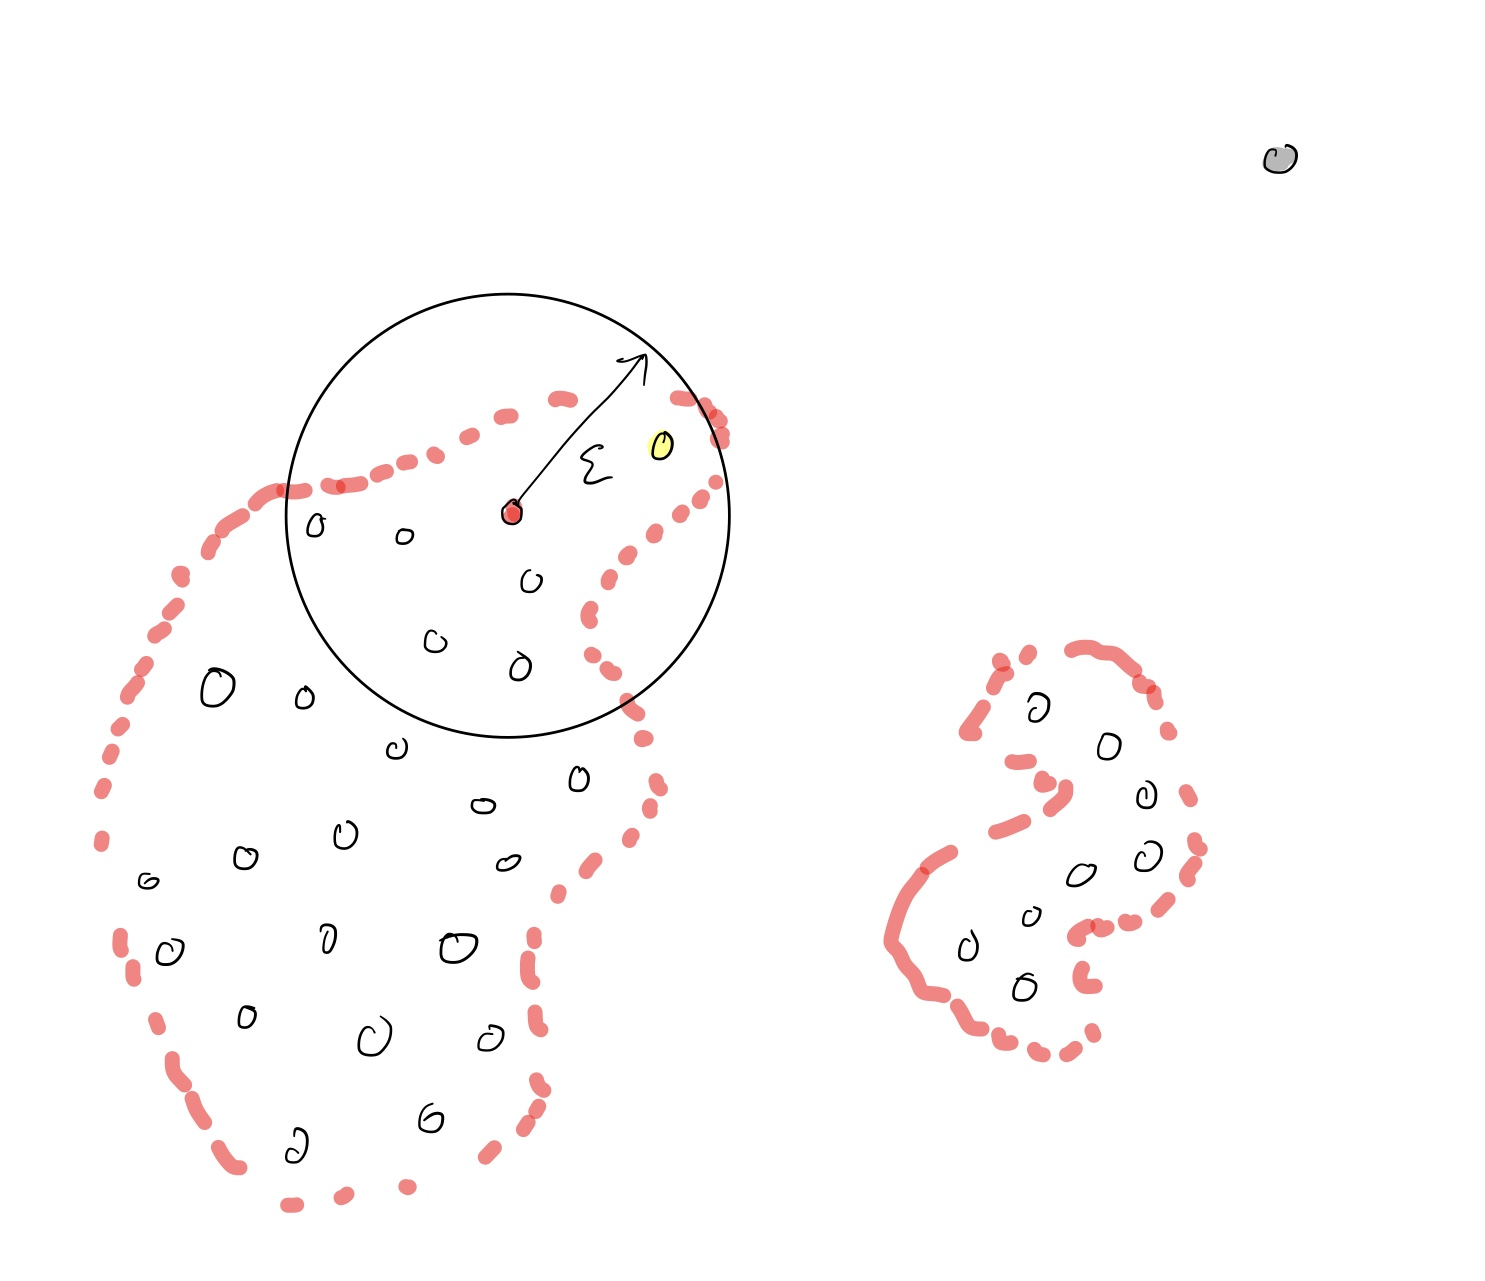
\includegraphics[width=.7\linewidth]{chapter_2/images/dbscan.jpg}
  \end{center}

  We can also see that if we take our core points as our vertices, put an edge between
  the core points that are close to each other and run connected components on
  the graph, then we will get precisely the two partitions above.

  \subsection{The algorithm}

  We include a formal definition of the algorithm:

  \begin{enumerate}
  \item Let $C=\{x \in X \ | \ X \cap B(x, \epsilon) \geq m\}$.
  \item Construct the graph $G=(V,E)$, with $V=C$, $E=\{(i,j) \ | \ ||x_i-x_j|| \leq \epsilon\}$.
  \item Run connected components on $G$. The clusters are the connected components
  \item Let $B=\{x \in X \ | \ x \notin C, \exists c \in C, ||x-c|| \leq \epsilon\}$.
  For each $b \in B$, assign $b$ to the connected component of any arbitrary $c$
  that is within $\epsilon$ of $b$.
  \item Ignore the rest of the points, which we consider noise points.

  \end{enumerate}
  \subsection{Pros and Cons}
  \subsection{Examples}
